% =====================================================================
\section{Introduzione}
\label{sec:intro}
% =====================================================================

Questa sezione costruisce il vocabolario necessario per leggere le
specifiche ETSI: parte dalla QKD come primitiva crittografica, passa alla
rete QKD con i suoi nodi fidati e la sua architettura a strati, richiama i
concetti essenziali di SDN e arriva infine ai due documenti che precedono la
GS~QKD~018: la GS~QKD~002 (§\ref{sec:qkd002}) e la GS~QKD~015
(§\ref{sec:qkd015}).

\paragraph{La distribuzione quantistica di chiavi.}

\begin{definition}[QKD]
La \emph{Quantum Key Distribution} è una procedura che, tramite il
trasporto di stati quantistici, consente a due parti remote di concordare
stringhe di bit segrete condivise, con una sicurezza basata
sull'entanglement o sull'impossibilità di clonare o misurare perfettamente
stati quantistici sconosciuti~\cite{qkd018}.
\end{definition}

L'idea si capisce bene con BB84. Alice codifica bit casuali su singoli
fotoni in una di due basi scelte a caso; Bob misura in una base anch'essa
casuale; su un canale classico \emph{autenticato} i due confrontano le basi
e tengono solo i bit misurati nella base giusta (\emph{sifting}). Un
intercettatore che misura i fotoni introduce inevitabilmente errori,
quantificati dal \emph{Quantum Bit Error Rate}
\begin{equation}
  \mathrm{QBER} = \frac{N_{\text{errori}}}{N_{\text{sifted}}} .
\end{equation}
Se il QBER resta sotto una soglia (circa l'$11\%$ per BB84 contro attacchi
collettivi), correzione d'errore e \emph{privacy amplification} distillano
una chiave segreta; altrimenti il blocco viene scartato. La grandezza che
interessa alla rete è il \emph{secret key rate} (SKR), cioè i bit di chiave
sicura prodotti al secondo. Poiché la trasmittanza della fibra decade come
$\eta = 10^{-\alpha L/10}$, con $\alpha \approx 0{,}2$~dB/km, anche l'SKR
cala rapidamente con la lunghezza $L$ del collegamento.

Due osservazioni, che ritroveremo nei casi d'uso della GS~QKD~002, sono
fondamentali. La QKD \emph{distribuisce} chiavi ma non cifra né autentica:
va sempre combinata con un cifrario (one-time pad o AES) e con un
meccanismo di autenticazione. Inoltre il canale classico deve essere
autenticato fin dal primo scambio, il che richiede un piccolo segreto
pre-condiviso: la QKD è quindi, a rigore, un meccanismo di \emph{key
growing}.

\paragraph{Dal link alla rete: il trusted node.}
Un link QKD copre al massimo qualche centinaio di chilometri e non esistono
ancora ripetitori quantistici pratici. Le reti reali collegano quindi i
link in serie tramite nodi fidati.

\begin{definition}[Trusted node e key relay]
Un \emph{trusted node} è un nodo, collocato in un perimetro fisicamente
protetto, che condivide chiavi QKD con entrambi i vicini. Per trasportare
una chiave $K$ da $A$ a $C$ passando per $B$, il nodo $A$ invia
$c = K \oplus K_{AB}$; $B$ calcola $K = c \oplus K_{AB}$ e inoltra
$c' = K \oplus K_{BC}$. Ogni hop è cifrato con \emph{one-time pad}, ma $K$
compare in chiaro dentro ciascun nodo intermedio, che deve quindi essere
fidato.
\end{definition}

Si noti che il relay consuma chiave: per trasportare $|K|$ bit lungo un
cammino $p$ ogni link $\ell\in p$ spende $|K|$ bit della propria chiave
locale. Questo semplice fatto rende la chiave una \emph{risorsa di rete} da
pianificare, ed è il motivo per cui le specifiche successive parlano di
tassi disponibili, consumi e cammini.

\paragraph{L'architettura a strati ITU-T.}
La raccomandazione ITU-T Y.3800~\cite{ituy3800} organizza una rete QKD
(QKDN) in strati sovrapposti (Fig.~\ref{fig:itu}): il \emph{quantum layer}
con i moduli QKD; il \emph{key management layer} con i key manager che
memorizzano e inoltrano le chiavi; il \emph{control layer}, che prende
decisioni operative (instradamento, relay, configurazione dei link); il
\emph{management layer}, che supervisiona il tutto; e il \emph{service
layer}, dove le applicazioni consumano le chiavi. In questo schema si
distinguono due tipi di collegamento.

\begin{definition}[QKD link e KM link]
Un \emph{QKD link} connette due moduli QKD ed è composto da canale
quantistico e canale classico: è il luogo in cui la chiave viene
\emph{generata}. Un \emph{KM link} connette due \emph{key manager} ed è il
canale classico, protetto con chiavi QKD, lungo il quale la chiave viene
\emph{inoltrata} (key relay).
\end{definition}

Allo stesso modo si distinguono due ruoli spesso confusi. Il \emph{QKDN
controller} agisce sulla rete in tempo reale: decide i cammini di relay,
attiva o disattiva link, reagisce ai guasti. Il \emph{QKDN manager} ha un
compito di supervisione: raccoglie informazioni FCAPS (\emph{Fault,
Configuration, Accounting, Performance, Security}) e applica politiche. Le
specifiche ETSI che vedremo si collocano nel piano di controllo: la
GS~QKD~015 tra controller e nodi, la GS~QKD~018 tra controller e
orchestrator.

% Figura: architettura a strati di una QKDN (ITU-T Y.3800)
\begin{figure}[t]
\centering
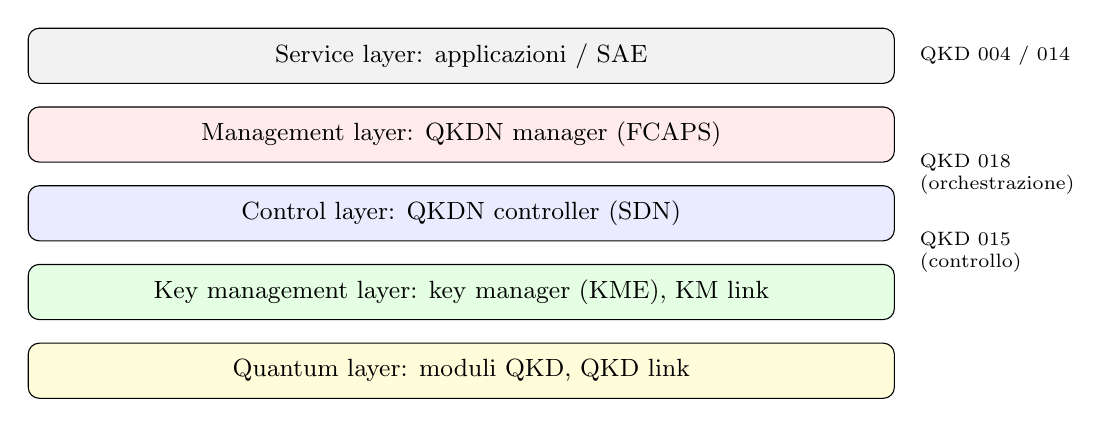
\begin{tikzpicture}[
  layer/.style={draw,rounded corners,minimum width=11cm,minimum height=7mm,
                align=center,font=\small},
  side/.style={font=\scriptsize,align=left,anchor=west}]
  \node[layer,fill=gray!10]   (srv) at (0,0)    {Service layer: applicazioni / SAE};
  \node[layer,fill=red!8]     (mgm) at (0,-1.0) {Management layer: QKDN manager (FCAPS)};
  \node[layer,fill=blue!8]    (ctl) at (0,-2.0) {Control layer: QKDN controller (SDN)};
  \node[layer,fill=green!10]  (km)  at (0,-3.0) {Key management layer: key manager (KME), KM link};
  \node[layer,fill=yellow!15] (q)   at (0,-4.0) {Quantum layer: moduli QKD, QKD link};
  \node[side] at (5.7,0)    {QKD 004 / 014};
  \node[side] at (5.7,-1.5) {QKD 018\\(orchestrazione)};
  \node[side] at (5.7,-2.5) {QKD 015\\(controllo)};
\end{tikzpicture}
\caption[Architettura a strati di una rete QKD (ITU-T Y.3800)]{Architettura a strati di una rete QKD secondo ITU-T
Y.3800~\cite{ituy3800}, con a destra la collocazione indicativa delle
specifiche ETSI discusse nel testo.}
\label{fig:itu}
\end{figure}


Le applicazioni non vedono la parte quantistica. Un \emph{Secure
Application Entity} (SAE) chiede chiavi al \emph{Key Management Entity}
(KME) del proprio nodo tramite le API GS~QKD~004~\cite{qkd004} o
GS~QKD~014~\cite{qkd014}; due SAE che vogliono comunicare ricevono la
stessa chiave dai rispettivi KME, identificata da un \emph{key ID}.

\paragraph{Software-Defined Networking.}
In una rete tradizionale ogni apparato decide da solo come instradare il
traffico. SDN~\cite{kreutz2015} separa invece tre piani: il \emph{piano
dati}, fatto di dispositivi che eseguono; il \emph{piano di controllo},
accentrato in un controller con la vista globale della rete; il
\emph{piano di gestione e applicazione}, che esprime gli obiettivi. Il
controller parla con i dispositivi tramite un'interfaccia
\emph{southbound} (SBI) e offre i propri servizi verso l'alto tramite
un'interfaccia \emph{northbound} (NBI). Quando i domini sono più di uno, si
aggiunge sopra i controller un \emph{orchestrator}, che coordina servizi
end-to-end senza conoscere i dettagli di ciascun dominio.

Una rete QKD ha tutte le caratteristiche che rendono utile SDN: risorse
scarse e variabili (la chiave), vincoli fisici stringenti (attenuazione,
coesistenza con canali classici), apparati di vendor diversi e domande che
cambiano nel tempo. Le due specifiche che seguono descrivono perché e come
l'ETSI ha applicato questo paradigma alla QKD.
